
\documentclass[12pt,a4paper]{report}

%% ─── Packages ────────────────────────────────────────────────────────────────
\usepackage[T1]{fontenc}
\usepackage[utf8]{inputenc}
\usepackage{lmodern}
\usepackage[margin=2.5cm]{geometry}
\usepackage{graphicx}
\usepackage{float}
\usepackage{listings}
\usepackage{xcolor}
\usepackage{hyperref}
\usepackage{booktabs}
\usepackage{array}
\usepackage{enumitem}
\usepackage{titlesec}
\usepackage{fancyhdr}
\usepackage{parskip}
\usepackage{tcolorbox}
\tcbuselibrary{listings,breakable,skins}

%% ─── Image path ──────────────────────────────────────────────────────────────
\graphicspath{{./image/}}

%% ─── Colours ─────────────────────────────────────────────────────────────────
\definecolor{k8sblue}{RGB}{50,100,200}
\definecolor{k8sgreen}{RGB}{15,157,99}
\definecolor{codebg}{RGB}{28,28,35}
\definecolor{codetext}{RGB}{220,220,220}
\definecolor{promptgreen}{RGB}{80,200,120}
\definecolor{warnbg}{RGB}{255,245,220}
\definecolor{warnborder}{RGB}{201,138,0}
\definecolor{notebg}{RGB}{235,245,255}
\definecolor{noteborder}{RGB}{50,100,200}
\definecolor{okbg}{RGB}{235,255,240}
\definecolor{okborder}{RGB}{15,157,99}

%% ─── Code listing style ──────────────────────────────────────────────────────
\lstdefinestyle{terminal}{
  backgroundcolor=\color{codebg},
  basicstyle=\ttfamily\footnotesize\color{codetext},
  breaklines=true,
  keepspaces=true,
  showstringspaces=false,
  frame=single,
  rulecolor=\color{k8sblue},
  framesep=6pt,
  xleftmargin=6pt,
  xrightmargin=6pt,
  aboveskip=8pt,
  belowskip=8pt,
}
\lstset{style=terminal}

%% ─── tcolorbox environments ──────────────────────────────────────────────────
\tcbset{
  warningbox/.style={
    colback=warnbg, colframe=warnborder,
    fonttitle=\bfseries, title={Warning},
    breakable, boxrule=0.8pt, left=6pt, right=6pt
  },
  notebox/.style={
    colback=notebg, colframe=noteborder,
    fonttitle=\bfseries, title={Explanation},
    breakable, boxrule=0.8pt, left=6pt, right=6pt
  },
  outputbox/.style={
    colback=okbg, colframe=okborder,
    fonttitle=\bfseries, title={Expected Output},
    breakable, boxrule=0.8pt, left=6pt, right=6pt
  },
}

%% ─── Page style ──────────────────────────────────────────────────────────────
\pagestyle{fancy}
\fancyhf{}
\fancyhead[L]{\small\textit{Cloud Computing Lab --- Kubernetes Hands-On}}
\fancyhead[R]{\small\textit{Neel Prajapati | 202611022}}
\fancyfoot[C]{\thepage}
\renewcommand{\headrulewidth}{0.4pt}

%% ─── Section formatting ──────────────────────────────────────────────────────
\titleformat{\chapter}[display]
  {\normalfont\Large\bfseries\color{k8sblue}}
  {Step \thechapter}{10pt}{\Huge}

\titleformat{\section}
  {\normalfont\large\bfseries\color{k8sblue}}
  {\thesection}{1em}{}

\titleformat{\subsection}
  {\normalfont\normalsize\bfseries\color{k8sgreen}}
  {\thesubsection}{1em}{}

%% ─── Hyperref setup ──────────────────────────────────────────────────────────
\hypersetup{
  colorlinks=true,
  linkcolor=k8sblue,
  urlcolor=k8sblue,
  citecolor=k8sblue,
  pdftitle={Kubernetes Hands-On Lab Report},
  pdfauthor={Neel Prajapati},
}

%% ─────────────────────────────────────────────────────────────────────────────
\begin{document}

%% ===========================================================================
%%  TITLE PAGE
%% ===========================================================================
\begin{titlepage}
  \centering
  \vspace*{1.5cm}

  {\Huge\bfseries\color{k8sblue} Lab Report}\\[0.5cm]
  {\large\color{gray} Cloud Computing}\\[2cm]

  \rule{\linewidth}{2pt}\\[0.5cm]
  {\LARGE\bfseries Kubernetes, Hands-On}\\[0.3cm]
  {\large\color{k8sgreen} 60-Minute Lab: Build, Deploy, Scale, Update \& Debug}\\[0.5cm]
  \rule{\linewidth}{2pt}\\[2cm]

  \begin{tabular}{rl}
    \textbf{Name:}           & Neel Prajapati \\[6pt]
    \textbf{Enrollment No.:} & 202611022 \\[6pt]
    \textbf{Subject:}        & Cloud Computing \\[6pt]
    \textbf{Lab URL:}        & \url{https://k8slabs.learnwithdutta.com/} \\[6pt]
    \textbf{Date:}           & 16 October 2026 \\
  \end{tabular}

  \vfill
  {\small Powered by: \textit{Learn with Gautam Dutta} $\cdot$ Kubernetes Hands-On Lab}
\end{titlepage}

%% ===========================================================================
%%  TABLE OF CONTENTS
%% ===========================================================================
\tableofcontents
\clearpage

%% ===========================================================================
%%  INTRODUCTION
%% ===========================================================================
\chapter*{Introduction}
\addcontentsline{toc}{chapter}{Introduction}

\section*{Objective}
This report documents the hands-on Kubernetes 60-minute lab performed on 16 October 2026.
The goals were to:
\begin{enumerate}[leftmargin=2em]
  \item Build a 3-node Kubernetes cluster on a local machine using \texttt{kind}.
  \item Inspect cluster components and understand control-plane vs.\ worker node roles.
  \item Deploy the first application (nginx) using a Deployment YAML manifest.
  \item Expose the application on a real browser port using a NodePort Service.
  \item Scale up/down replicas and observe self-healing behaviour.
  \item Update the application image and perform a rollback.
  \item Deliberately break the cluster and diagnose the error.
\end{enumerate}

\section*{What is Kubernetes?}
Kubernetes is \textbf{a program you give a wish to. It then works non-stop to make that wish true.}

Unlike Docker (which executes a single \texttt{docker run} command), Kubernetes accepts a
\textbf{standing instruction}: ``keep three copies of this app running''. It continuously monitors
the cluster and repairs deviations --- analogous to a thermostat set to a fixed temperature.

\section*{Key Terminology}
\begin{center}
\begin{tabular}{>{\bfseries}lp{9.5cm}}
\toprule
Term & Meaning \\
\midrule
Cluster       & A group of machines managed as one unit. \\
Node          & One machine (here: a Docker container acting as a server). \\
Control Plane & The master node that stores configuration and schedules Pods. \\
Worker        & A node that actually runs application Pods. \\
Pod           & One running copy of an app --- disposable, replaced frequently. \\
Deployment    & The instruction: ``keep N copies of this image running''. \\
Service       & One stable address in front of changing Pods, matched by labels. \\
\bottomrule
\end{tabular}
\end{center}

\section*{Lab Plan}
\begin{center}
\begin{tabular}{cll}
\toprule
Time & Step & Achievement \\
\midrule
0--10 min  & Setup              & Built a Kubernetes cluster on a laptop \\
10--15 min & 1. Look at cluster  & Understood the three-node architecture \\
15--26 min & 2. Run first app    & Wrote one YAML; Kubernetes spread it on two machines \\
26--37 min & 3. Open in browser  & App accessible on a real port (30000) \\
37--44 min & 4. Scale \& kill    & Deleted running app; nothing went down \\
44--52 min & 5. Update \& undo   & Shipped new version and rolled it back \\
52--60 min & 6. Break \& fix     & Read an error and found the root cause \\
\bottomrule
\end{tabular}
\end{center}

\clearpage

%% ===========================================================================
%%  SETUP
%% ===========================================================================
\chapter*{Setup --- Building the Cluster}
\addcontentsline{toc}{chapter}{Setup --- Building the Cluster}

\section*{Tool Verification}
\begin{lstlisting}
$ docker ps
$ kubectl version --client
$ kind version
\end{lstlisting}

\section*{Working Directory}
\begin{lstlisting}
$ mkdir -p ~/k8s-lab && cd ~/k8s-lab
\end{lstlisting}

\section*{Generate Configuration and Build the Cluster}
The shell block below writes \texttt{kind-config.yaml} (one control-plane, two workers,
ports 30000--30050 mapped for browser access), then creates the cluster:

\begin{lstlisting}
$ {
  echo 'kind: Cluster'
  echo 'apiVersion: kind.x-k8s.io/v1alpha4'
  echo 'name: k8s-lab'
  echo 'nodes:'
  echo '  - role: control-plane'
  echo '    extraPortMappings:'
  for p in $(seq 30000 30050); do
    echo "      - containerPort: $p"
    echo "        hostPort: $p"
    echo "        protocol: TCP"
  done
  echo '  - role: worker'
  echo '  - role: worker'
} > kind-config.yaml

$ kind create cluster --config kind-config.yaml
\end{lstlisting}

\begin{figure}[H]
  \centering
  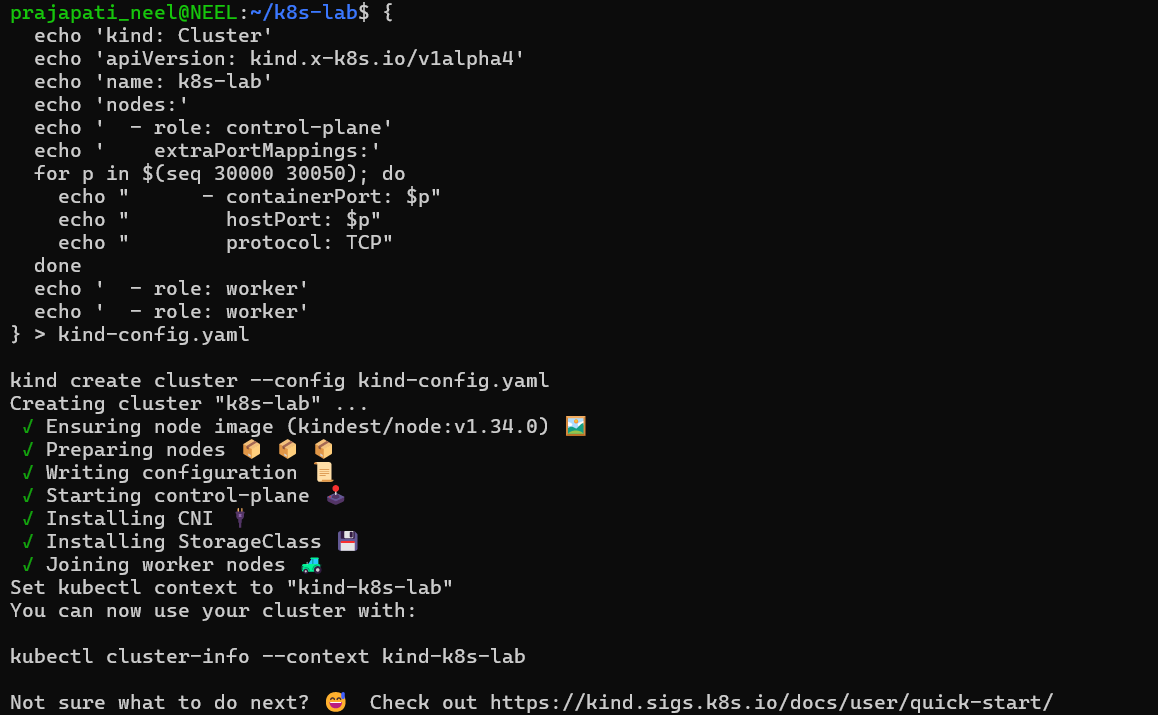
\includegraphics[width=0.92\textwidth]{Screenshot 2026-10-16 185920.png}
  \caption{Setup --- Creating the kind cluster. The configuration is written and \texttt{kind create cluster} runs successfully, completing all phases: Ensuring node image, Preparing nodes, Writing configuration, Starting control-plane, Installing CNI, Installing StorageClass, and Joining worker nodes.}
\end{figure}

\section*{Verify Nodes}
\begin{lstlisting}
$ kubectl get nodes
$ docker ps --format "{{.Names}}"
\end{lstlisting}

\begin{figure}[H]
  \centering
  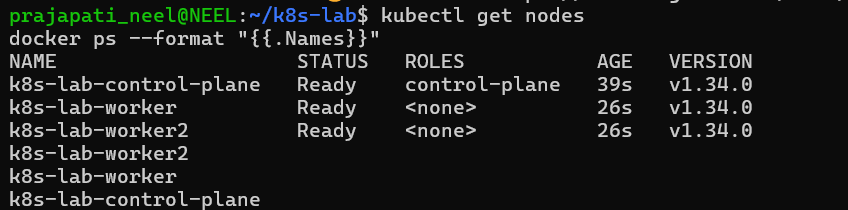
\includegraphics[width=0.92\textwidth]{Screenshot 2026-10-16 185928.png}
  \caption{Setup --- All three nodes (\texttt{k8s-lab-control-plane}, \texttt{k8s-lab-worker}, \texttt{k8s-lab-worker2}) are \texttt{Ready} running Kubernetes v1.34.0.}
\end{figure}

\begin{tcolorbox}[notebox]
\textbf{kind} = ``Kubernetes IN Docker''. It runs a full cluster inside containers on a laptop.
Cleanup is simple: deleting the cluster means deleting three Docker containers.
\end{tcolorbox}

\clearpage

%% ===========================================================================
%%  STEP 1
%% ===========================================================================
\chapter{Look at Your Cluster}
\textit{Goal: Meet the three machines and see Kubernetes running itself.}
\hfill \textbf{\textasciitilde5 min | Easy}

\section{Checking the Current Context and Nodes}
\begin{lstlisting}
$ kubectl config current-context
$ kubectl get nodes -o wide
$ kubectl get pods
\end{lstlisting}

\begin{figure}[H]
  \centering
  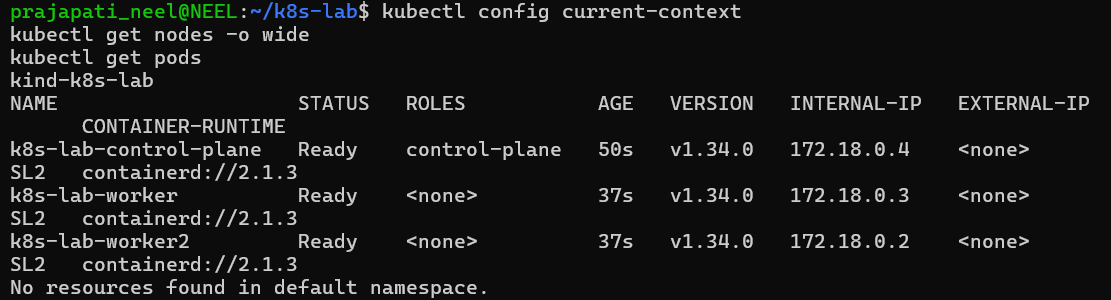
\includegraphics[width=0.95\textwidth]{Screenshot 2026-10-16 185943.png}
  \caption{Step 1 --- Current context is \texttt{kind-k8s-lab}. Nodes listed with internal IPs and container runtime (containerd 2.1.3). \texttt{kubectl get pods} returns ``No resources found in default namespace'' --- correct, nothing deployed yet.}
\end{figure}

\begin{tcolorbox}[notebox]
``No resources found'' is \textbf{correct, not an error.}
Always verify your context (\texttt{kubectl config current-context}) before running destructive commands.
\end{tcolorbox}

\section{Why Apps Never Run on the Control Plane}
\begin{lstlisting}
$ kubectl describe node k8s-lab-control-plane | grep -i -A1 taints
\end{lstlisting}

\begin{tcolorbox}[outputbox]
\begin{lstlisting}[style=terminal,colback=okbg]
Taints: node-role.kubernetes.io/control-plane:NoSchedule
\end{lstlisting}
\end{tcolorbox}

A \textbf{taint} is a ``keep out'' sign. Without a matching toleration in the Pod spec,
the scheduler never places application Pods on the control plane --- preventing a rogue app
from consuming control-plane resources.

\section{System Pods in kube-system}
\begin{lstlisting}
$ kubectl get pods -n kube-system -o wide
\end{lstlisting}

\begin{figure}[H]
  \centering
  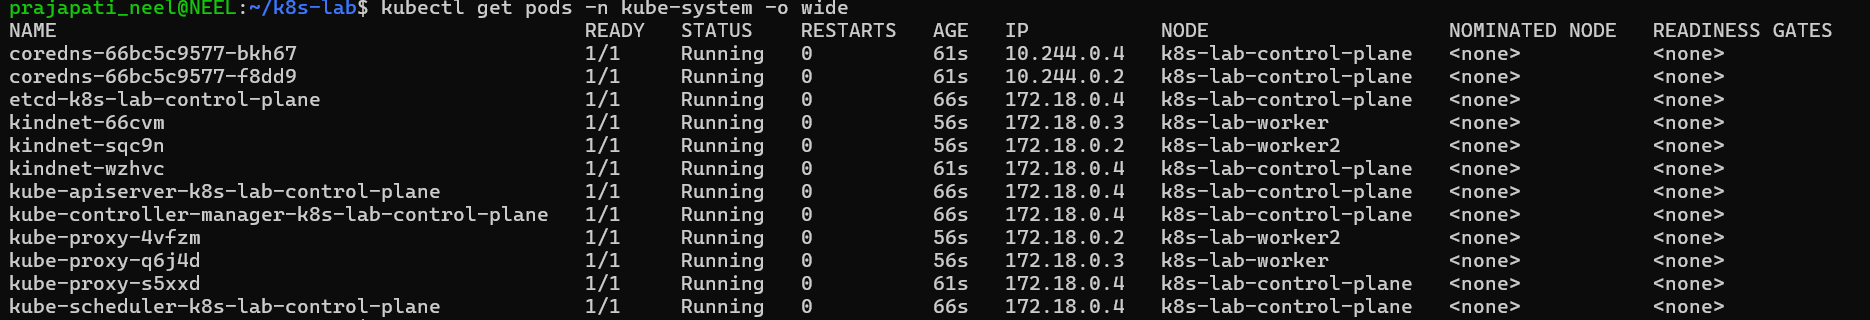
\includegraphics[width=0.99\textwidth]{Screenshot 2026-10-16 185959.png}
  \caption{Step 1 --- System pods in the \texttt{kube-system} namespace. All are \texttt{Running} with 0 restarts. Control-plane pods (\texttt{etcd}, \texttt{kube-apiserver}, \texttt{kube-controller-manager}, \texttt{kube-scheduler}, \texttt{coredns}) run only on the control-plane node. Networking pods (\texttt{kube-proxy}, \texttt{kindnet}) run on all three nodes.}
\end{figure}

\begin{center}
\begin{tabular}{lll}
\toprule
Pod & Where & Job \\
\midrule
\texttt{kube-apiserver}          & control plane      & Front door --- all commands go here \\
\texttt{etcd}                    & control plane      & The notebook --- stores everything \\
\texttt{kube-scheduler}          & control plane      & Chooses which node runs each new Pod \\
\texttt{kube-controller-manager} & control plane      & The thermostat --- desired vs.\ actual \\
\texttt{coredns}                 & control plane      & DNS resolution inside the cluster \\
\texttt{kube-proxy, kindnet}     & all three nodes    & Networking (one copy per node) \\
\bottomrule
\end{tabular}
\end{center}

\clearpage

%% ===========================================================================
%%  STEP 2
%% ===========================================================================
\chapter{Run Your First App}
\textit{Goal: Write one file. Watch Kubernetes build three objects and place them on two machines.}
\hfill \textbf{\textasciitilde11 min | The main one}

\section{Creating the Deployment YAML}
\begin{lstlisting}
$ nano deployment.yaml
\end{lstlisting}

\begin{lstlisting}
apiVersion: apps/v1
kind: Deployment
metadata:
  name: nginx
spec:
  replicas: 3
  selector:
    matchLabels:
      app: nginx
  template:
    metadata:
      labels:
        app: nginx
    spec:
      containers:
        - name: nginx
          image: nginx:stable
          ports:
            - containerPort: 80
          resources:
            requests:
              cpu: "50m"
              memory: "64Mi"
\end{lstlisting}

\begin{center}
\begin{tabular}{lp{8.5cm}}
\toprule
Field & Meaning \\
\midrule
\texttt{kind: Deployment}    & Type of wish: keep copies of an app running. \\
\texttt{replicas: 3}         & \textbf{The dial.} Three copies, always. \\
\texttt{app: nginx} (twice)  & Label sticker. Deployment and Service both use it. \\
\texttt{template}            & Cookie-cutter --- describes one Pod. \\
\texttt{image: nginx:stable} & Which container image to pull. \\
\texttt{requests}            & CPU/memory reservation. \texttt{50m} = 5\% of one core. \\
\bottomrule
\end{tabular}
\end{center}

\section{Applying the Deployment}
\begin{lstlisting}
$ kubectl apply --dry-run=client -f deployment.yaml
$ kubectl apply -f deployment.yaml
$ kubectl wait --for=condition=Available deployment/nginx --timeout=120s
$ kubectl get pods -o wide
\end{lstlisting}

\begin{figure}[H]
  \centering
  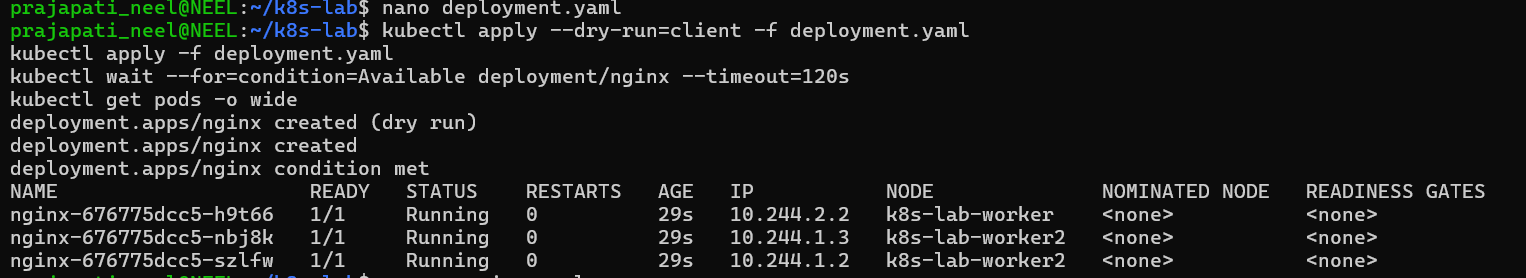
\includegraphics[width=0.99\textwidth]{Screenshot 2026-10-16 190011.png}
  \caption{Step 2 --- Dry-run passes, deployment created, and \texttt{kubectl wait} confirms \texttt{condition met}. Three nginx pods (\texttt{nginx-676775dcc5-h9t66}, \texttt{-nbj8k}, \texttt{-szlfw}) are \texttt{Running} across both worker nodes.}
\end{figure}

\begin{tcolorbox}[notebox]
\textbf{Look at the NODE column.} You never chose a machine; the \textit{scheduler} decided.
The Pods are spread across \texttt{k8s-lab-worker} and \texttt{k8s-lab-worker2} automatically.
\end{tcolorbox}

\section{One File, Three Objects}
\begin{lstlisting}
$ kubectl get deployments
$ kubectl get replicasets
$ kubectl get pods
\end{lstlisting}

\begin{itemize}
  \item \textbf{Deployment} --- what you wrote; manages rolling updates.
  \item \textbf{ReplicaSet} --- created for you; ensures exactly 3 Pods exist at all times.
  \item \textbf{Pod} --- created by the ReplicaSet; one running copy with its own IP.
\end{itemize}

You created \textbf{one} object. Kubernetes built the other two and maintains them forever.

\clearpage

%% ===========================================================================
%%  STEP 3
%% ===========================================================================
\chapter{Open it in a Browser}
\textit{Goal: Give three moving Pods one fixed address, then reach it on a real port.}
\hfill \textbf{\textasciitilde11 min | Easy | The payoff}

\section{Creating the Service YAML}
\begin{lstlisting}
$ nano service.yaml
\end{lstlisting}

\begin{lstlisting}
apiVersion: v1
kind: Service
metadata:
  name: nginx
spec:
  type: NodePort
  selector:
    app: nginx
  ports:
    - protocol: TCP
      port: 80          # the Service's port inside the cluster
      targetPort: 80    # the port inside the container
      nodePort: 30000   # the port you type in your browser
\end{lstlisting}

\section{Applying the Service and Checking Endpoints}
\begin{lstlisting}
$ kubectl apply -f service.yaml
$ kubectl get services
$ kubectl get endpoints nginx
\end{lstlisting}

\begin{figure}[H]
  \centering
  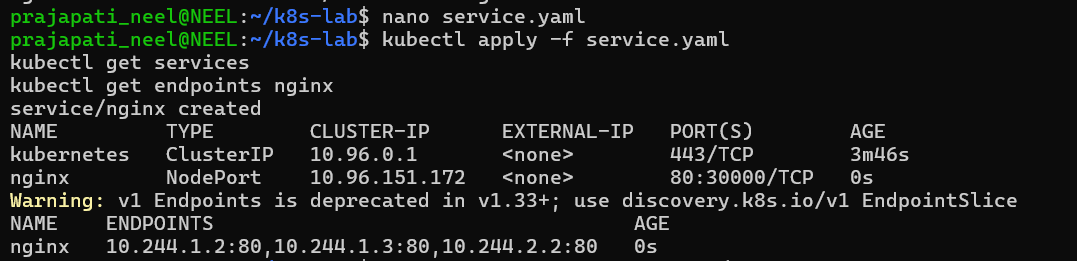
\includegraphics[width=0.95\textwidth]{Screenshot 2026-10-16 190021.png}
  \caption{Step 3 --- Service applied. \texttt{kubectl get services} shows the nginx NodePort Service on \texttt{80:30000/TCP}. \texttt{kubectl get endpoints nginx} lists three endpoints (one per Pod) at their respective IPs --- proof that label matching worked.}
\end{figure}

\begin{tcolorbox}[warningbox]
\texttt{selector: app: nginx} must exactly match the label in \texttt{deployment.yaml}.
A mismatch produces zero endpoints and silent failures --- the most common Kubernetes bug.
\end{tcolorbox}

\section{Visiting the App in the Browser}
Navigate to \textbf{\texttt{http://localhost:30000}} in a browser:

\begin{figure}[H]
  \centering
  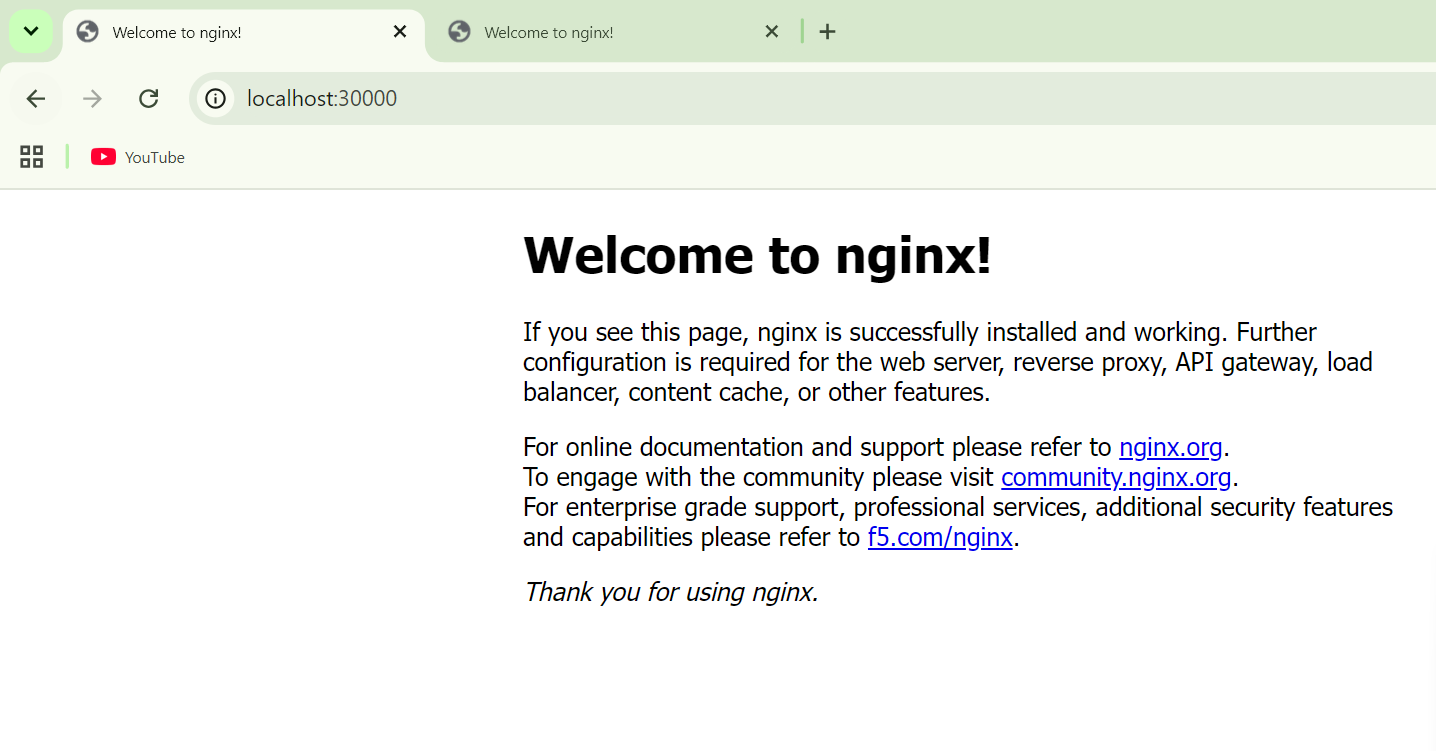
\includegraphics[width=0.85\textwidth]{Screenshot 2026-10-16 175436.png}
  \caption{Step 3 --- The \textbf{``Welcome to nginx!''} page is displayed at \texttt{localhost:30000}. The NodePort Service is forwarding traffic from the control-plane node through to a running Pod on a worker node.}
\end{figure}

\section{Port Mapping Summary}
\begin{center}
\begin{tabular}{llp{7cm}}
\toprule
Field & Lives on & Purpose \\
\midrule
\texttt{nodePort: 30000} & every node  & External port; must be 30000--32767. \\
\texttt{port: 80}        & the Service & Internal cluster port for other Pods. \\
\texttt{targetPort: 80}  & the Pod     & Port the container actually listens on. \\
\bottomrule
\end{tabular}
\end{center}

\section{Quick Tunnel Alternative}
\begin{lstlisting}
$ kubectl port-forward service/nginx 8080:80
\end{lstlisting}

\begin{figure}[H]
  \centering
  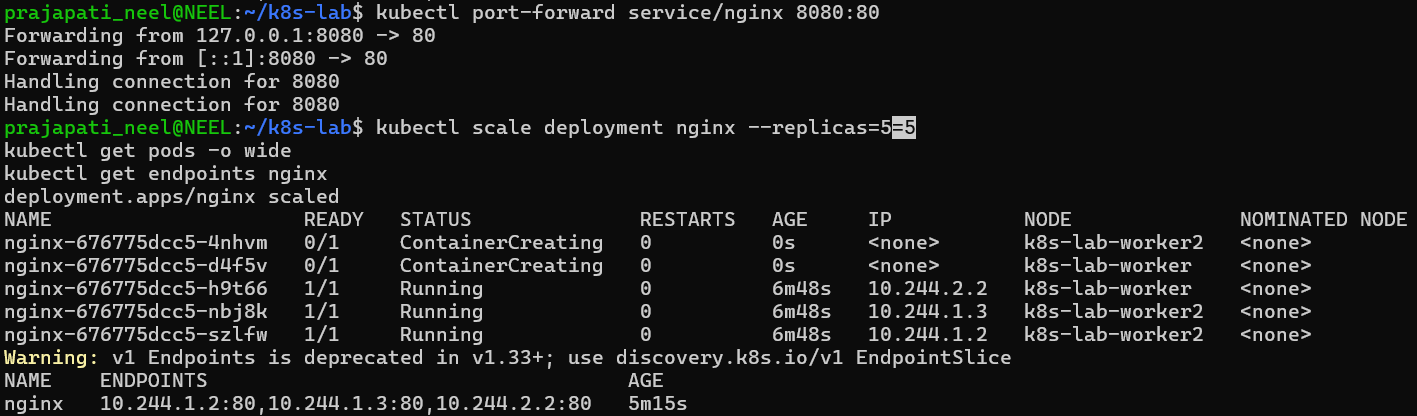
\includegraphics[width=0.95\textwidth]{Screenshot 2026-10-16 190036.png}
  \caption{Step 3 / 4 combined --- \texttt{kubectl port-forward} active in one terminal while \texttt{kubectl scale --replicas=5} is run in another. The scaling shows two new pods in \texttt{ContainerCreating}. Endpoints still show only the original three until new pods become Ready.}
\end{figure}

\clearpage

%% ===========================================================================
%%  STEP 4
%% ===========================================================================
\chapter{Scale It, Then Kill It}
\textit{Goal: Turn the dial up, then delete a running Pod and watch nothing bad happen.}
\hfill \textbf{\textasciitilde7 min | Easy | The fun one}

\section{Scale Up to 5 Replicas}
\begin{lstlisting}
$ kubectl scale deployment nginx --replicas=5
$ kubectl get pods -o wide
$ kubectl get endpoints nginx
\end{lstlisting}

Two new Pods appeared. The original three were \textbf{not restarted}.
The Service automatically picked up the new Pods by label --- \texttt{service.yaml} was untouched.

\section{Scale Back Down to 3}
\begin{lstlisting}
$ kubectl scale deployment nginx --replicas=3
$ kubectl get pods -o wide -w
\end{lstlisting}

\begin{figure}[H]
  \centering
  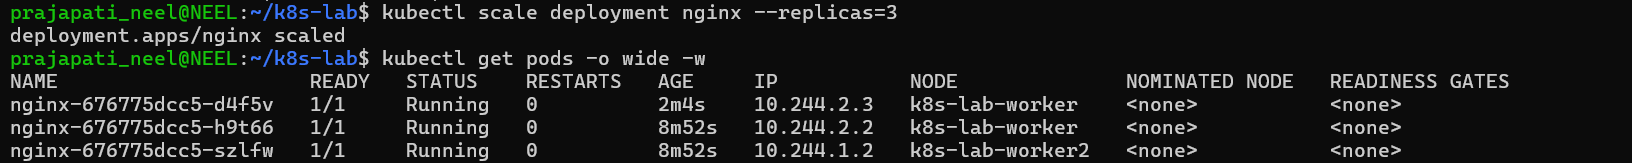
\includegraphics[width=0.95\textwidth]{Screenshot 2026-10-16 190055.png}
  \caption{Step 4 --- After scaling back to 3. All three Pods are \texttt{Running} and distributed across both worker nodes (\texttt{k8s-lab-worker} and \texttt{k8s-lab-worker2}).}
\end{figure}

\section{Deliberately Deleting a Pod}
\begin{lstlisting}
$ kubectl get pods
\end{lstlisting}

\begin{figure}[H]
  \centering
  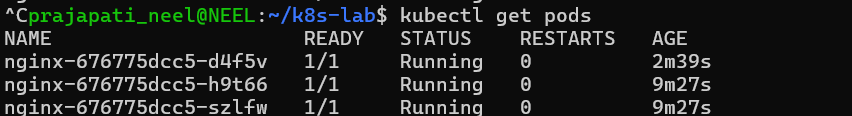
\includegraphics[width=0.92\textwidth]{Screenshot 2026-10-16 190104.png}
  \caption{Step 4 --- Three pods listed before deletion. Pod \texttt{nginx-676775dcc5-szlfw} was selected for deletion to demonstrate self-healing.}
\end{figure}

\begin{lstlisting}
$ kubectl delete pod nginx-676775dcc5-szlfw
\end{lstlisting}

Within approximately 2 seconds a new Pod with a new name and new IP appears, placed by the
scheduler on whichever node has capacity. The site never went down --- the two surviving
Pods served all requests during the replacement.

\begin{tcolorbox}[notebox]
\textbf{That is the thermostat working.} The ReplicaSet counted 2 Pods, wanted 3, and created one more.
This is why Pods are called \textbf{disposable} --- never write a Pod IP address into application code.
The Service exists precisely because Pod IPs always change.
\end{tcolorbox}

\begin{tcolorbox}[warningbox]
To really remove the app, change the \textit{wish}: \texttt{kubectl delete deployment nginx}.
Deleting individual Pods only causes the ReplicaSet to create replacements.
\end{tcolorbox}

\clearpage

%% ===========================================================================
%%  STEP 5
%% ===========================================================================
\chapter{Update, Redeploy, Undo}
\textit{Goal: Ship a new version with zero downtime, force a redeploy, then take it all back.}
\hfill \textbf{\textasciitilde8 min | Medium}

\section{5.1 --- Imperative Update}
\begin{lstlisting}
$ kubectl set image deployment/nginx nginx=nginx:stable-alpine
$ kubectl rollout status deployment/nginx
\end{lstlisting}

\begin{figure}[H]
  \centering
  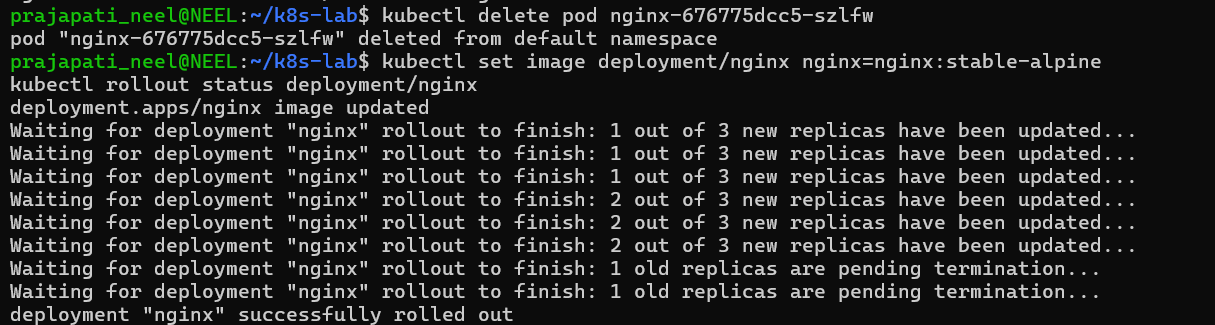
\includegraphics[width=0.99\textwidth]{Screenshot 2026-10-16 190111.png}
  \caption{Step 5.1 --- Imperative image update to \texttt{nginx:stable-alpine}. Rolling update: 1 new replica updated, then 2, then old replicas terminate. Final message: ``deployment \texttt{nginx} successfully rolled out''. The site remained accessible throughout.}
\end{figure}

\section{5.2 --- Declarative Update}
Edit \texttt{deployment.yaml} to change the image and resource requests:

\begin{lstlisting}
$ nano deployment.yaml     # change image to burgxy/webapps:v4
$ kubectl apply -f deployment.yaml
$ kubectl rollout status deployment/nginx
\end{lstlisting}

\begin{figure}[H]
  \centering
  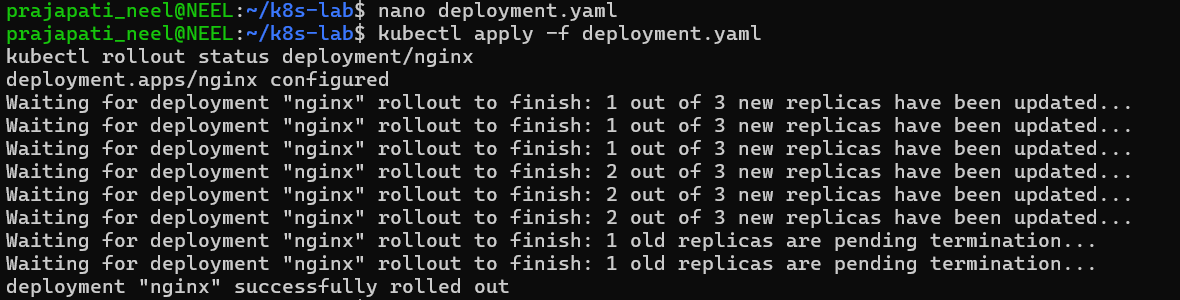
\includegraphics[width=0.99\textwidth]{Screenshot 2026-10-16 190149.png}
  \caption{Step 5.2 --- Declarative \texttt{kubectl apply -f deployment.yaml}. Status shows \texttt{configured} and the rolling update completes successfully. This approach is standard in production --- changes live in Git and are reproducible.}
\end{figure}

After the update, \texttt{kubectl get replicasets} shows \textbf{two ReplicaSets}:
the new one is active; the old one is empty but retained as the \textbf{undo button}.

\section{5.3 --- Rollback}
\begin{lstlisting}
$ kubectl rollout undo deployment/nginx
$ kubectl rollout status deployment/nginx
\end{lstlisting}

\section{5.4 --- Idempotent Apply (Nothing Changed)}
\begin{lstlisting}
$ kubectl apply -f deployment.yaml
\end{lstlisting}

\begin{figure}[H]
  \centering
  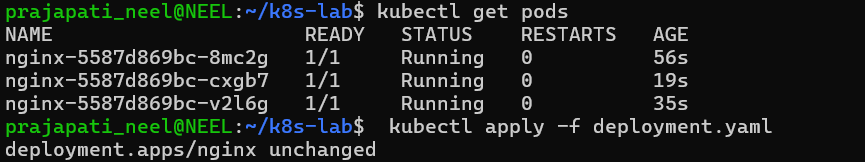
\includegraphics[width=0.92\textwidth]{Screenshot 2026-10-16 190158.png}
  \caption{Step 5.4 --- After the update, three pods from the new ReplicaSet (\texttt{nginx-5587d869bc-*}) are \texttt{Running}. Applying the same unchanged YAML returns \texttt{deployment.apps/nginx unchanged} --- \texttt{apply} is fully idempotent.}
\end{figure}

\begin{tcolorbox}[warningbox]
\textbf{Do not redeploy by deleting all Pods.} \texttt{kubectl delete pod -l app=nginx} removes every copy at once --- users see errors for seconds. Use \texttt{kubectl rollout restart deployment/nginx} instead; it replaces Pods one at a time with zero downtime.
\end{tcolorbox}

\clearpage

%% ===========================================================================
%%  STEP 6
%% ===========================================================================
\chapter{Break It and Fix It}
\textit{Goal: Cause a real failure, find the cause in 30 seconds, and repair it.}
\hfill \textbf{\textasciitilde8 min | The useful one}

\section{6.1 --- Deliberately Break the Deployment}
\begin{lstlisting}
$ kubectl set image deployment/nginx nginx=nginx:this-tag-does-not-exist
\end{lstlisting}

Wait 20 seconds:
\begin{lstlisting}
$ kubectl get pods
$ curl -s http://localhost:30000 | head -n 1
\end{lstlisting}

\begin{tcolorbox}[notebox]
The old Pods kept running and kept serving. The update \textit{stopped} instead of destroying
a working app. \textbf{A failed deployment is not automatically an outage.}
\end{tcolorbox}

\section{6.2 --- Diagnose with \texttt{describe}}
\begin{lstlisting}
$ kubectl describe pod <broken-pod-name>
\end{lstlisting}

\begin{figure}[H]
  \centering
  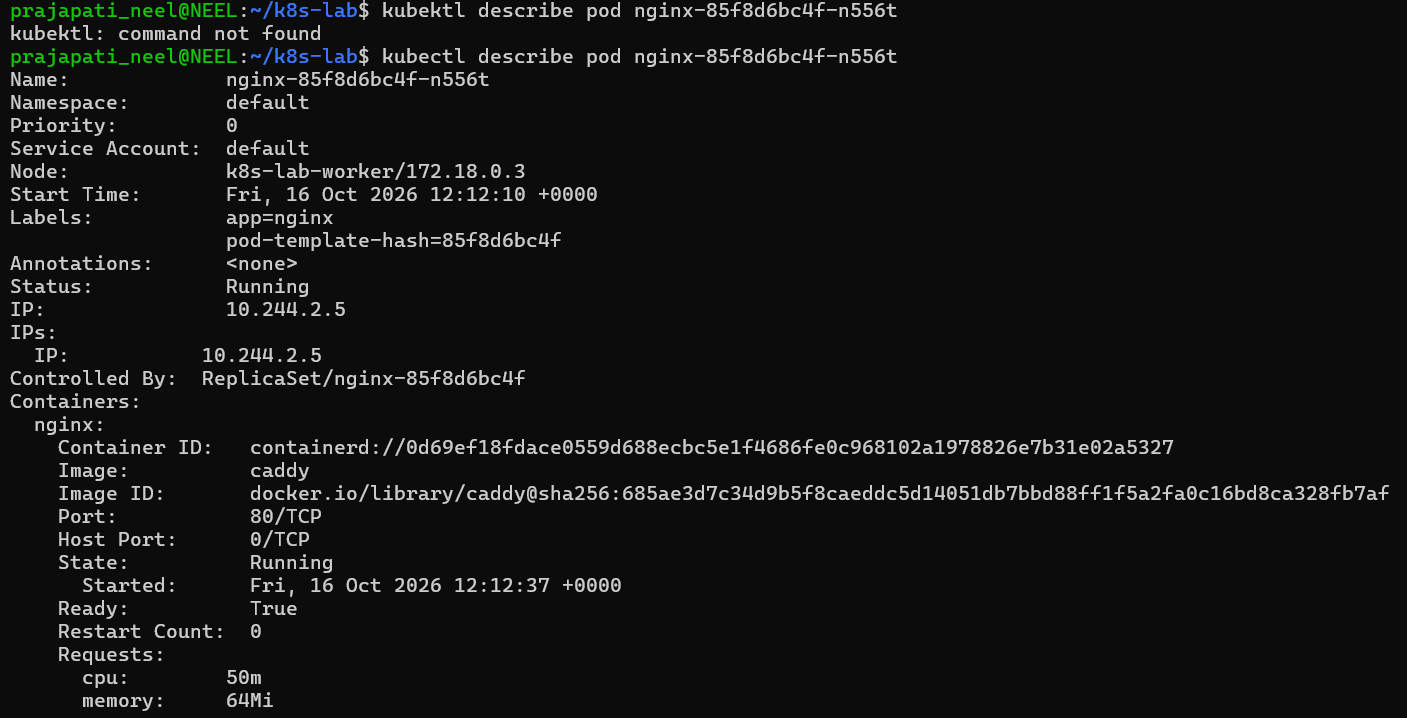
\includegraphics[width=0.99\textwidth]{Screenshot 2026-10-16 190124.png}
  \caption{Step 6 --- \texttt{kubectl describe pod} on the broken pod. Full metadata visible: Pod assigned to \texttt{k8s-lab-worker}, Status \texttt{Running}, Labels, Container details (image: caddy, Port: 80/TCP). Events section at bottom shows the full lifecycle trace.}
\end{figure}

\begin{figure}[H]
  \centering
  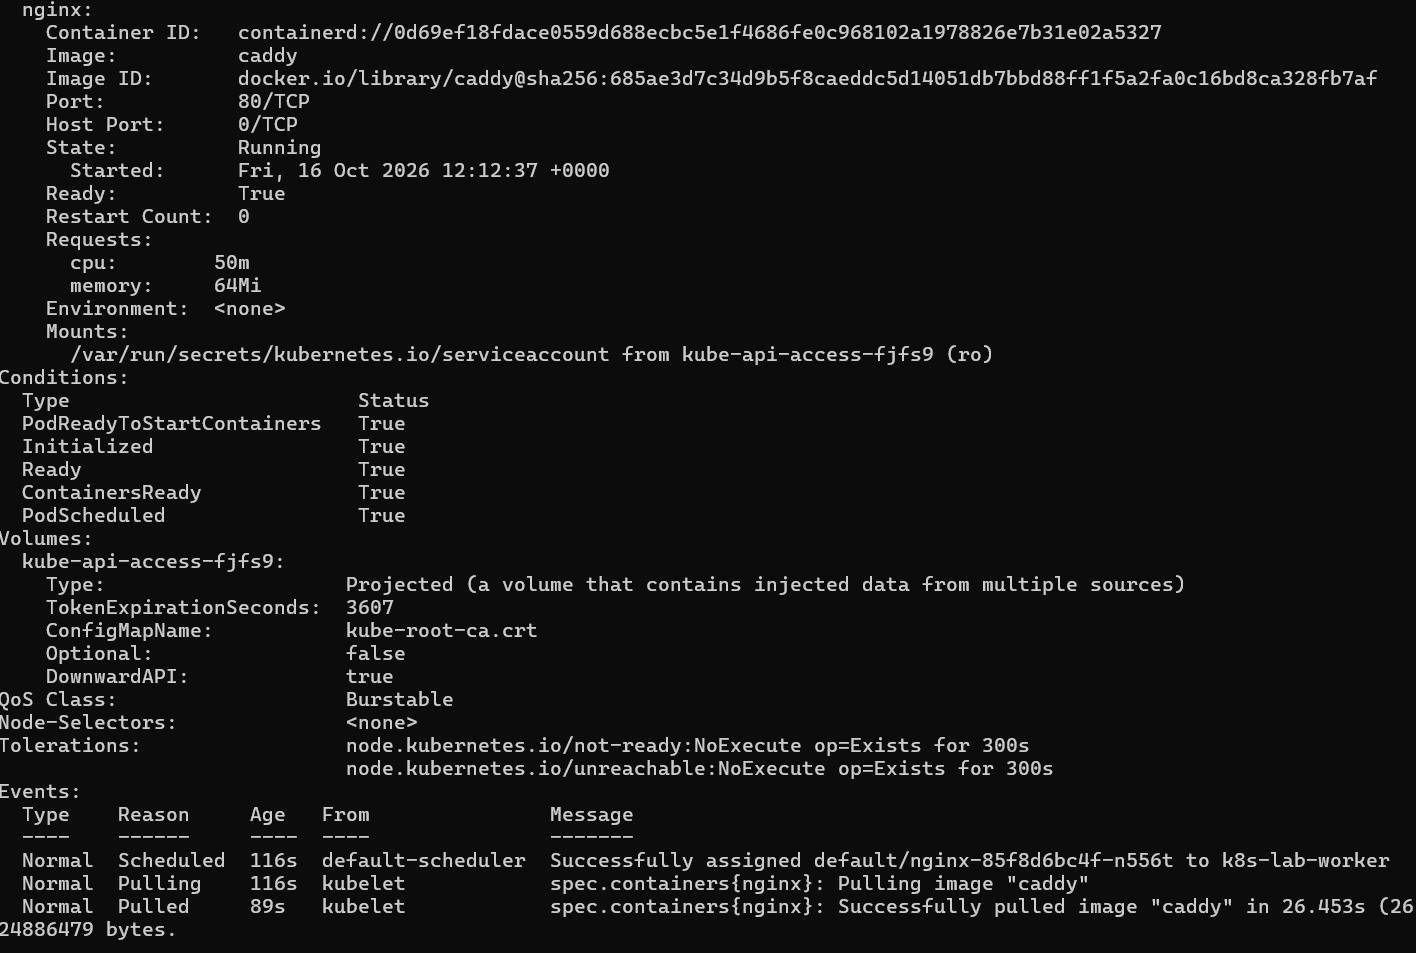
\includegraphics[width=0.99\textwidth]{Screenshot 2026-10-16 190137.png}
  \caption{Step 6 --- Continuation of \texttt{kubectl describe pod}. Container conditions all \texttt{True}, Volumes, QoS Class (\texttt{Burstable}), Tolerations, and Events: Scheduled $\to$ Pulling $\to$ Pulled (26s) $\to$ Running. For a broken pod the Events section would instead show \texttt{Failed} and \texttt{ImagePullBackOff}.}
\end{figure}

The Events section gives the answer in plain English:
\begin{enumerate}
  \item \texttt{Scheduled} --- scheduler placed the Pod successfully.
  \item \texttt{Pulling} --- kubelet started pulling the image.
  \item \texttt{Failed} --- image not found (wrong tag).
  \item \texttt{ImagePullBackOff} --- Kubernetes backs off, retrying with increasing delays.
\end{enumerate}

\section{6.3 --- Try \texttt{logs} (and understand why it fails here)}
\begin{lstlisting}
$ kubectl logs <broken-pod-name>
\end{lstlisting}

\begin{tcolorbox}[outputbox]
\begin{lstlisting}[style=terminal,colback=okbg]
Error from server (BadRequest): container "nginx" is waiting to start:
trying and failing to pull image
\end{lstlisting}
\end{tcolorbox}

\begin{tcolorbox}[notebox]
\textbf{The debugging rule:}\\
Use \textbf{\texttt{describe}} when the container \textit{never started} (image issues, scheduling failures).\\
Use \textbf{\texttt{logs}} when the container \textit{started but behaves wrongly} (application crashes, bad config).
\end{tcolorbox}

\section{6.4 --- Fix It}
\begin{lstlisting}
$ kubectl rollout undo deployment/nginx
$ kubectl rollout status deployment/nginx
$ kubectl get pods -o wide
$ kubectl get endpoints nginx
\end{lstlisting}

\textbf{Success criteria:} 3/3 Pods \texttt{Running}, three endpoints, and \texttt{http://localhost:30000} still serving the nginx page.

\begin{center}
\begin{tabular}{lll}
\toprule
Status & Root Cause & First Command \\
\midrule
\texttt{Pending}              & No node had sufficient resources & \texttt{kubectl describe pod NAME} \\
\texttt{ContainerCreating}    & Image being pulled (normal)      & Wait; if stuck, \texttt{describe} \\
\texttt{ImagePullBackOff}     & Wrong image name or tag          & \texttt{kubectl describe pod NAME} \\
\texttt{CrashLoopBackOff}     & App starts then crashes          & \texttt{kubectl logs NAME --previous} \\
\texttt{Running} but 0/1      & Alive, not passing readiness     & \texttt{kubectl describe pod NAME} \\
\texttt{Running}, user errors & Label mismatch, no endpoints     & \texttt{kubectl get endpoints NAME} \\
\bottomrule
\end{tabular}
\end{center}

\clearpage

%% ===========================================================================
%%  BONUS
%% ===========================================================================
\chapter*{Bonus: Declarative Image Update Result}
\addcontentsline{toc}{chapter}{Bonus: Declarative Image Update Result}

During Step 5's declarative update, the image was changed to use the \textbf{Caddy} web server.
After a successful zero-downtime rolling update, the browser confirmed the new application:

\begin{figure}[H]
  \centering
  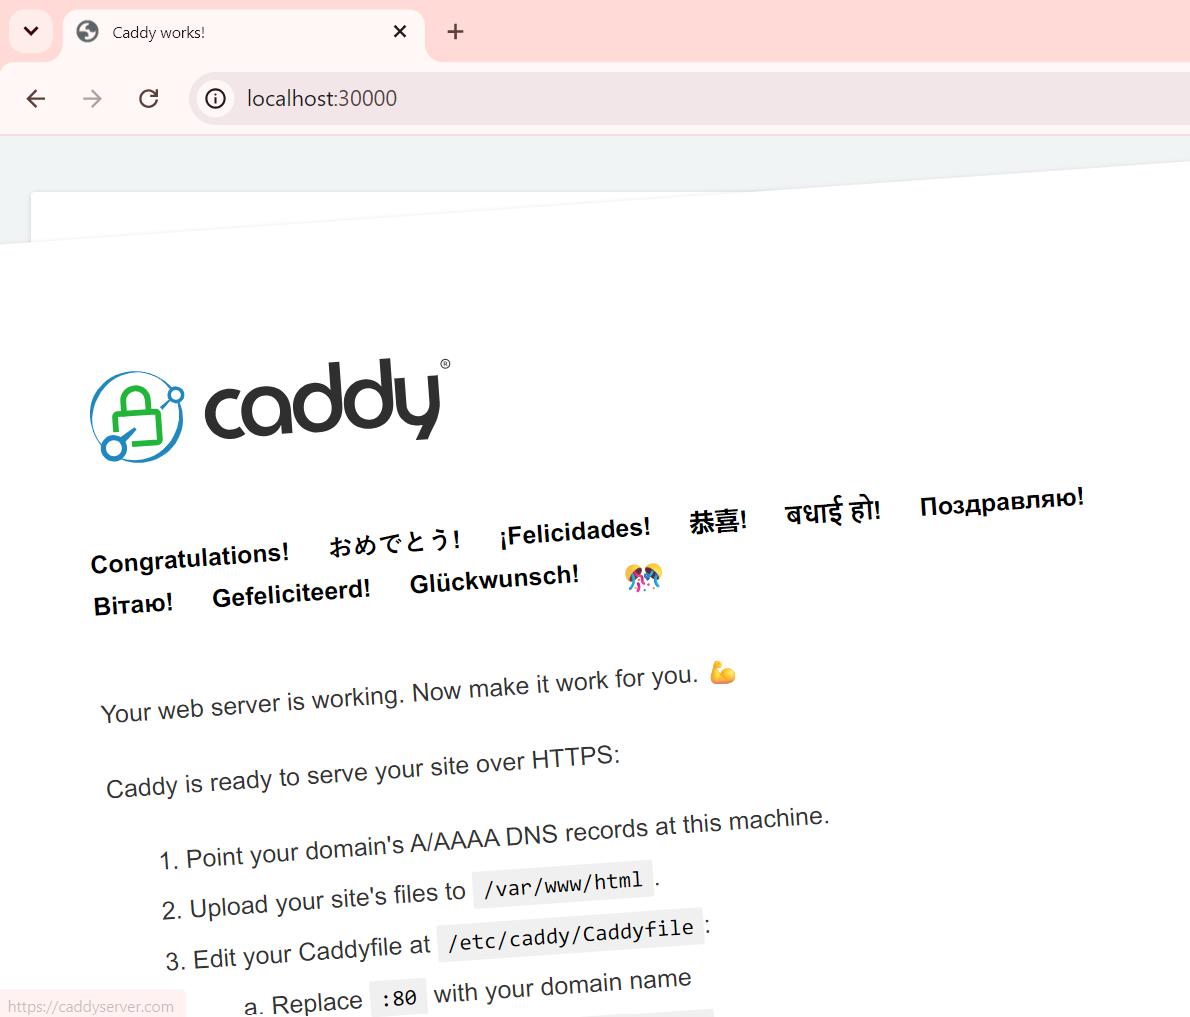
\includegraphics[width=0.80\textwidth]{Screenshot 2026-10-16 190225.png}
  \caption{Caddy web server running at \texttt{localhost:30000} after the rolling update. The page reads ``Your web server is working. Now make it work for you.'' --- confirming the Kubernetes rolling update mechanism replaced all Pods without downtime.}
\end{figure}

\clearpage

%% ===========================================================================
%%  CLEANUP
%% ===========================================================================
\chapter*{Cleanup}
\addcontentsline{toc}{chapter}{Cleanup}

\section*{Option A --- Remove the App, Keep the Cluster}
\begin{lstlisting}
$ kubectl delete -f service.yaml
$ kubectl delete -f deployment.yaml
$ kubectl get all
\end{lstlisting}
Only the built-in \texttt{kubernetes} Service remains.

\section*{Option B --- Delete the Entire Cluster}
\begin{lstlisting}
$ kind delete cluster --name k8s-lab
$ kind get clusters     # prints nothing
\end{lstlisting}

\begin{figure}[H]
  \centering
  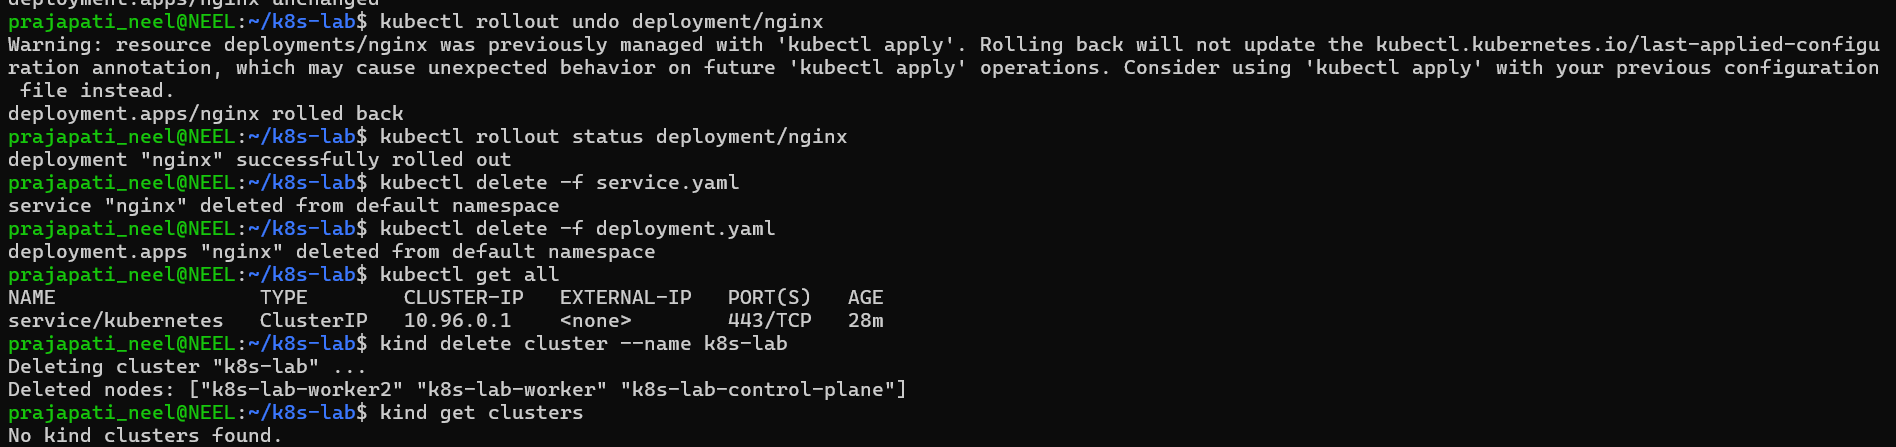
\includegraphics[width=0.99\textwidth]{Screenshot 2026-10-16 190209.png}
  \caption{Cleanup --- \texttt{kubectl rollout undo} completes the rollback, then \texttt{kubectl delete -f service.yaml} and \texttt{kubectl delete -f deployment.yaml} remove the app. \texttt{kubectl get all} confirms only the built-in \texttt{service/kubernetes} remains. Finally, \texttt{kind delete cluster --name k8s-lab} deletes all three container nodes and \texttt{kind get clusters} returns nothing.}
\end{figure}

\clearpage

%% ===========================================================================
%%  SUMMARY AND CONCLUSION
%% ===========================================================================
\chapter*{Summary and Conclusion}
\addcontentsline{toc}{chapter}{Summary and Conclusion}

\section*{Six Things Learned}
\begin{enumerate}[leftmargin=2em]
  \item \textbf{Kubernetes is a thermostat for software.} Write the desired state; Kubernetes
        continuously reconciles reality to match it.

  \item \textbf{One control plane, two workers.} A taint keeps apps off the control plane,
        preventing a rogue app from making the cluster unmanageable.

  \item \textbf{One YAML $\rightarrow$ three objects.} A single Deployment produced a
        Deployment, a ReplicaSet, and three Pods on two machines never explicitly named.
        \texttt{created} means ``wish saved'', not ``app running''.

  \item \textbf{Services find Pods by label.} A Service is a stable address in front of
        ephemeral Pods. \texttt{kubectl get endpoints} is the proof labels matched.

  \item \textbf{Deleting a Pod does not delete an app.} Only changing the desired state does.
        Use \texttt{rollout restart} for safe, zero-downtime Pod replacement.

  \item \textbf{Debugging rule:} \texttt{describe} when it never started; \texttt{logs} when
        it started but behaves wrongly. A failed update is not automatically an outage.
\end{enumerate}

\section*{Key Commands Reference}
\begin{center}
\begin{tabular}{ll}
\toprule
Goal & Command \\
\midrule
Check which cluster you are on (always do first!) & \texttt{kubectl config current-context} \\
See everything created                             & \texttt{kubectl get all} \\
See Pods with IPs and nodes                        & \texttt{kubectl get pods -o wide} \\
Watch changes live                                 & \texttt{kubectl get pods -w} \\
Find why something is unhappy                      & \texttt{kubectl describe pod NAME} \\
Read app output                                    & \texttt{kubectl logs NAME} \\
Check a Service found its Pods                     & \texttt{kubectl get endpoints NAME} \\
Change the number of copies                        & \texttt{kubectl scale deployment NAME --replicas=N} \\
Ship a new image                                   & \texttt{kubectl set image deployment/NAME c=img:tag} \\
Replace all Pods safely                            & \texttt{kubectl rollout restart deployment/NAME} \\
Undo the last change                               & \texttt{kubectl rollout undo deployment/NAME} \\
Validate YAML before applying                      & \texttt{kubectl apply --dry-run=client -f file.yaml} \\
\bottomrule
\end{tabular}
\end{center}

\section*{Conclusion}
This 60-minute lab provided full hands-on experience with core Kubernetes workflows used
in real production environments: cluster creation, declarative deployment, service exposure,
horizontal scaling, rolling updates, and fault diagnosis.

The key insight is the \textbf{declarative model}: express \textit{what} you want, not
\textit{how} to achieve it. Kubernetes then continuously reconciles actual state with
desired state, delivering self-healing, zero-downtime deployments, and safe rollbacks
as built-in features --- not scripts to maintain.

\vfill
\begin{center}
\rule{0.5\linewidth}{0.4pt}\\[0.3cm]
{\small \textit{Kubernetes Hands-On --- 60-Minute Lab}\\
\textit{Neel Prajapati} $\;|\;$ \textit{Enrollment No.: 202611022} $\;|\;$ \textit{Cloud Computing}}
\end{center}

\end{document}
